\documentclass{beamer}

%%%%%%%%%%%%%Solarized Theme%%%%%%%%%%%%%%%
\usecolortheme[dark,accent=cyan]{solarized}
\beamertemplatenavigationsymbolsempty
%%%%%Packages%%%%%
\usefonttheme{serif}
\usepackage[T1]{fontenc}
\usepackage[utf8]{inputenc}
\usepackage[english]{babel}
\usepackage{fontawesome}
\usepackage{minted}
\usepackage{soul}

\definecolor{DarkGray}{gray}{0.1}
\usemintedstyle{paraiso-dark}


\usepackage{graphicx}
\usepackage{hyperref}
\usepackage{colortbl, xcolor}
\usepackage{booktabs}
\usepackage{amsmath,amsthm, amssymb, latexsym}

\usepackage{tikz}
\usepackage{xcolor}
\usepackage{graphicx,multirow}
\definecolor{plain}{rgb}{93,93,93}
\usetikzlibrary{positioning,arrows}
\definecolor{applegreen}{rgb}{0.55, 0.71, 0.0}
\usetikzlibrary{decorations.pathreplacing, backgrounds, fit}
\usetikzlibrary{calc,matrix}

\tikzstyle{background}=[solarizedRed, rectangle, draw, inner sep=1mm, thick,
           rounded corners=2mm]

\usepackage{standalone}
\usepackage{siunitx}

\begin{document}

\begin{frame}
    \begin{center}
        \large{\textcolor{orange}{Web scraping, text analysis, and networks can help us identify the most important Avenger}} \\

        \vspace{1cm}
        \normalsize{@NikoletaGlyn}

    \end{center}
\end{frame}

\begin{frame}
    \begin{center}
    
\includegraphics[width=0.24\textwidth]{static/mpi.jpg}\hspace{8pt}
    
\includegraphics[width=0.24\textwidth]{static/python.png}\vspace{8pt}

    
\includegraphics[width=0.24\textwidth]{static/namibia.jpg}\hspace{8pt}
    
\includegraphics[width=0.24\textwidth]{static/django_girls.png}
    \end{center}
\end{frame}

\begin{frame}
    \hspace{.8cm} \LARGE{Marvel Comics} \\

    \hspace{.8cm} \normalsize{1. An American media and entertainment company}

    \hspace{1cm}\normalsize{that was widely regarded as one of the “big two”}

    \hspace{1cm}\normalsize{publishers in the comic industry.}
\end{frame}

\begin{frame}
    \hspace{.8cm} \LARGE{Marvel Cinematic Universe} \\

    \hspace{.8cm} \normalsize{1. Media franchise centered on a series of superhero films.}

    \hspace{1cm}\normalsize{The films are based on characters that appear in the}

    \hspace{1cm}\normalsize{comic books published by Marvel Comics.}
\end{frame}


\begin{frame}
    \begin{minipage}{.4\textwidth}
        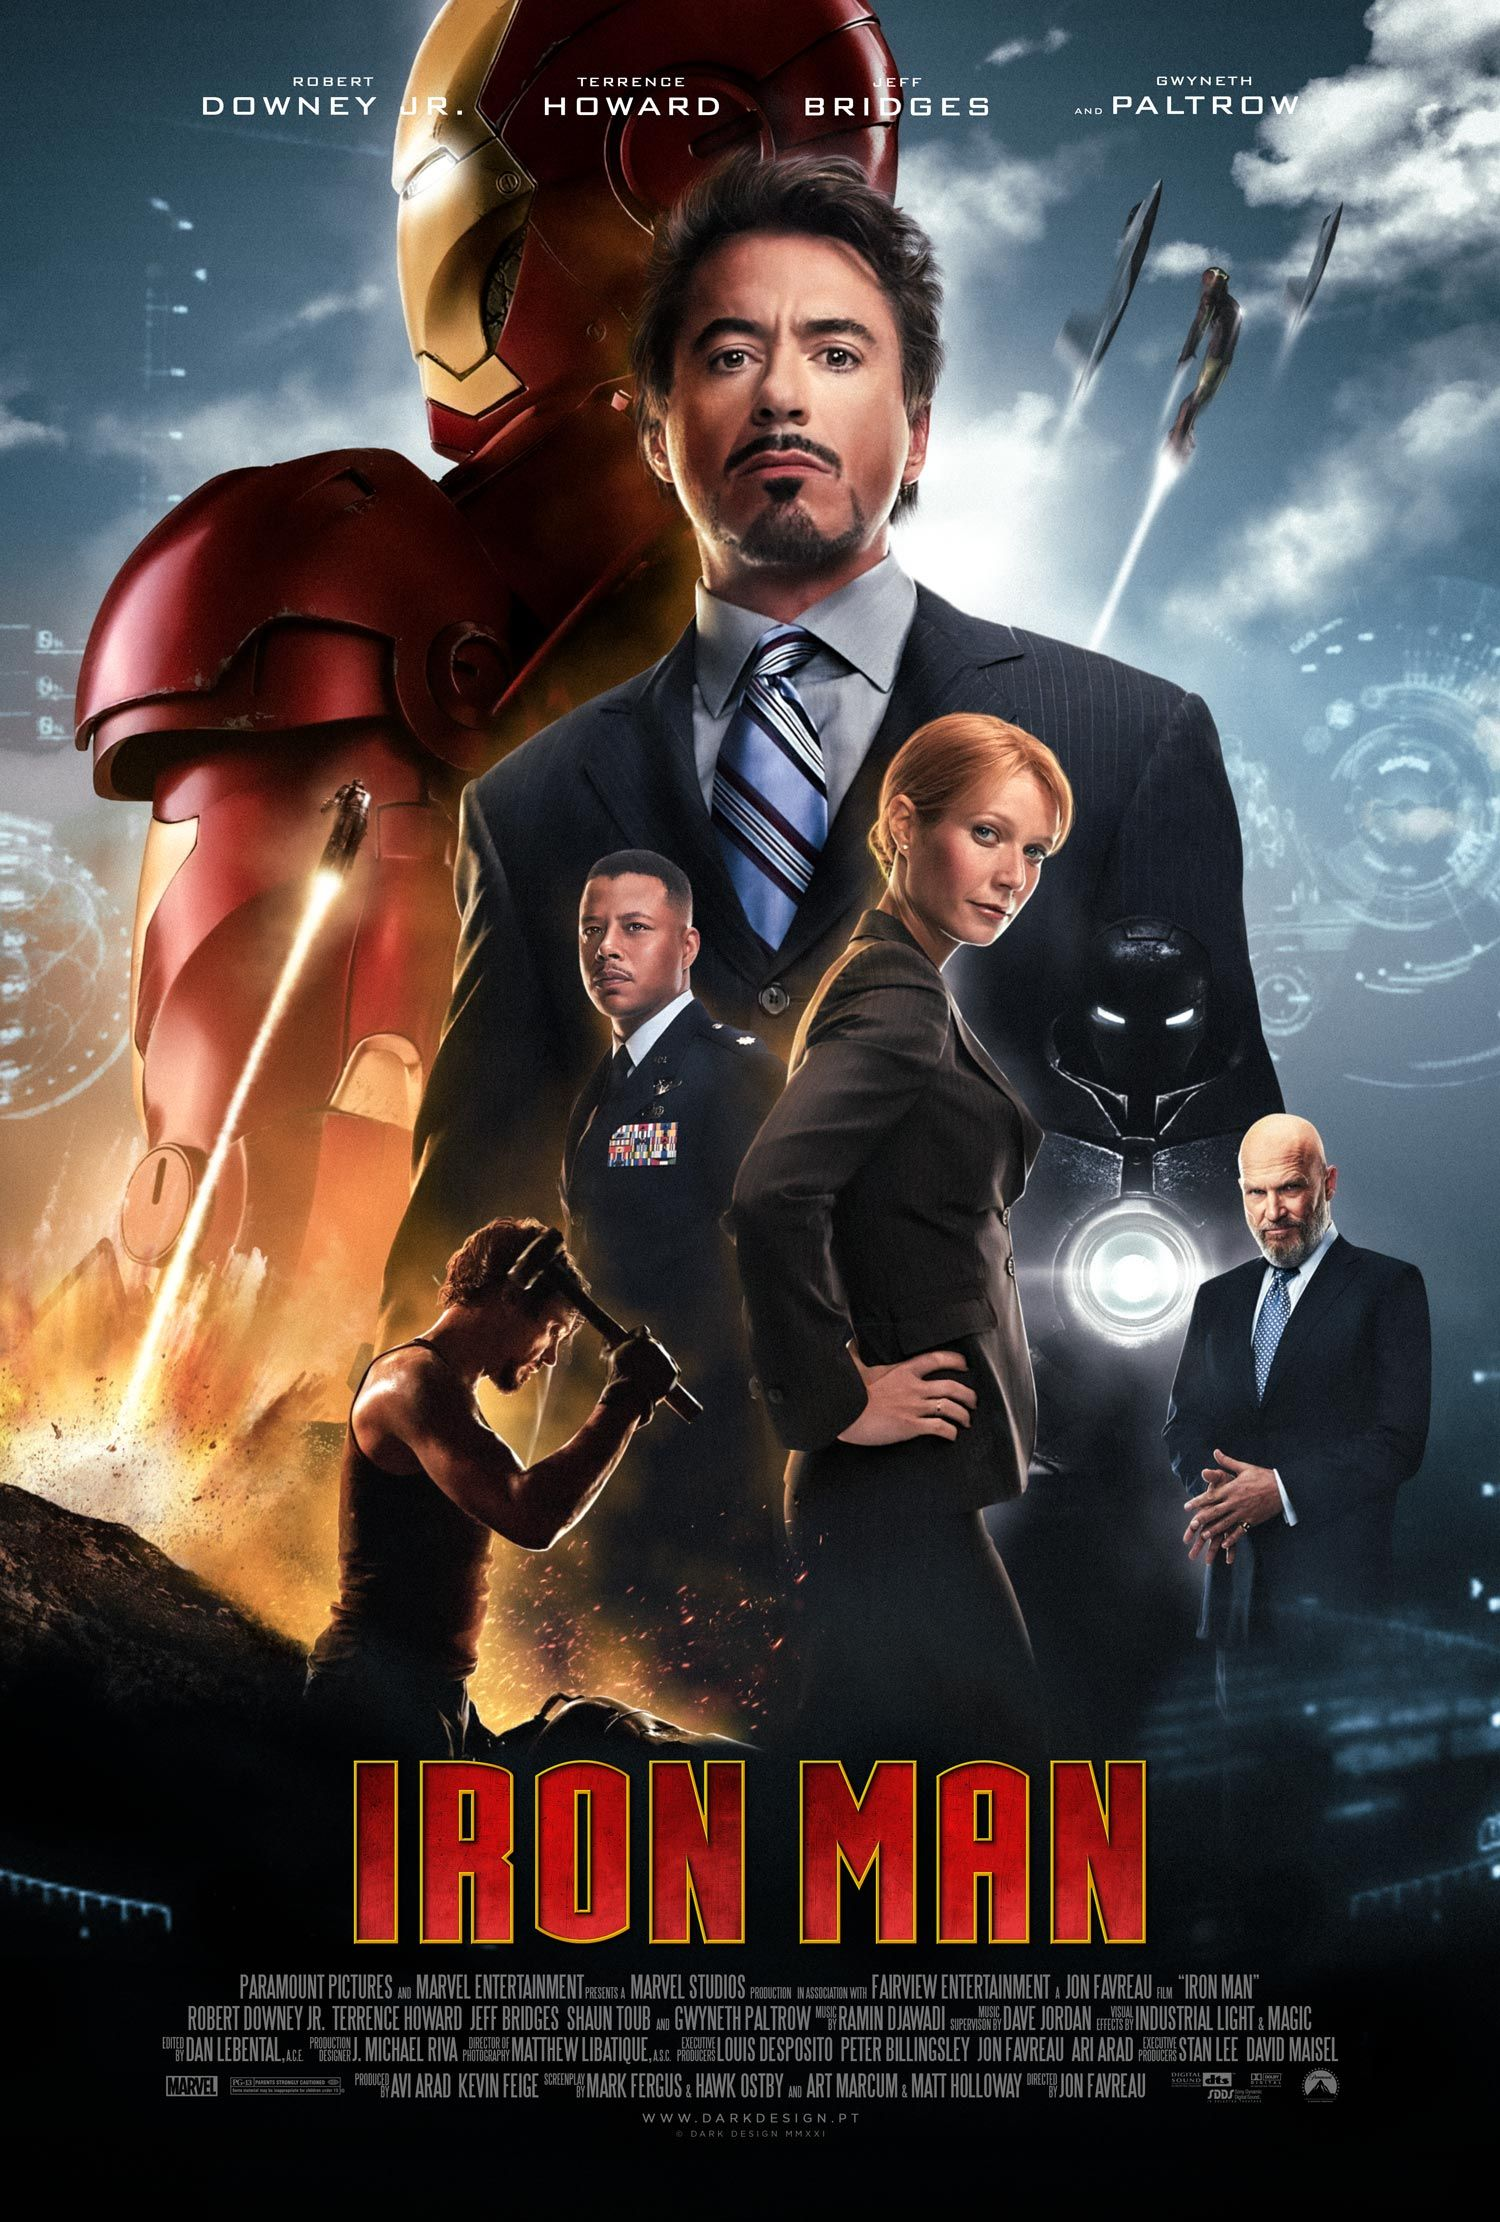
\includegraphics[width=.75\textwidth]{static/iron_man_2008.jpg}
    \end{minipage} \pause
    \begin{minipage}{.58\textwidth}
        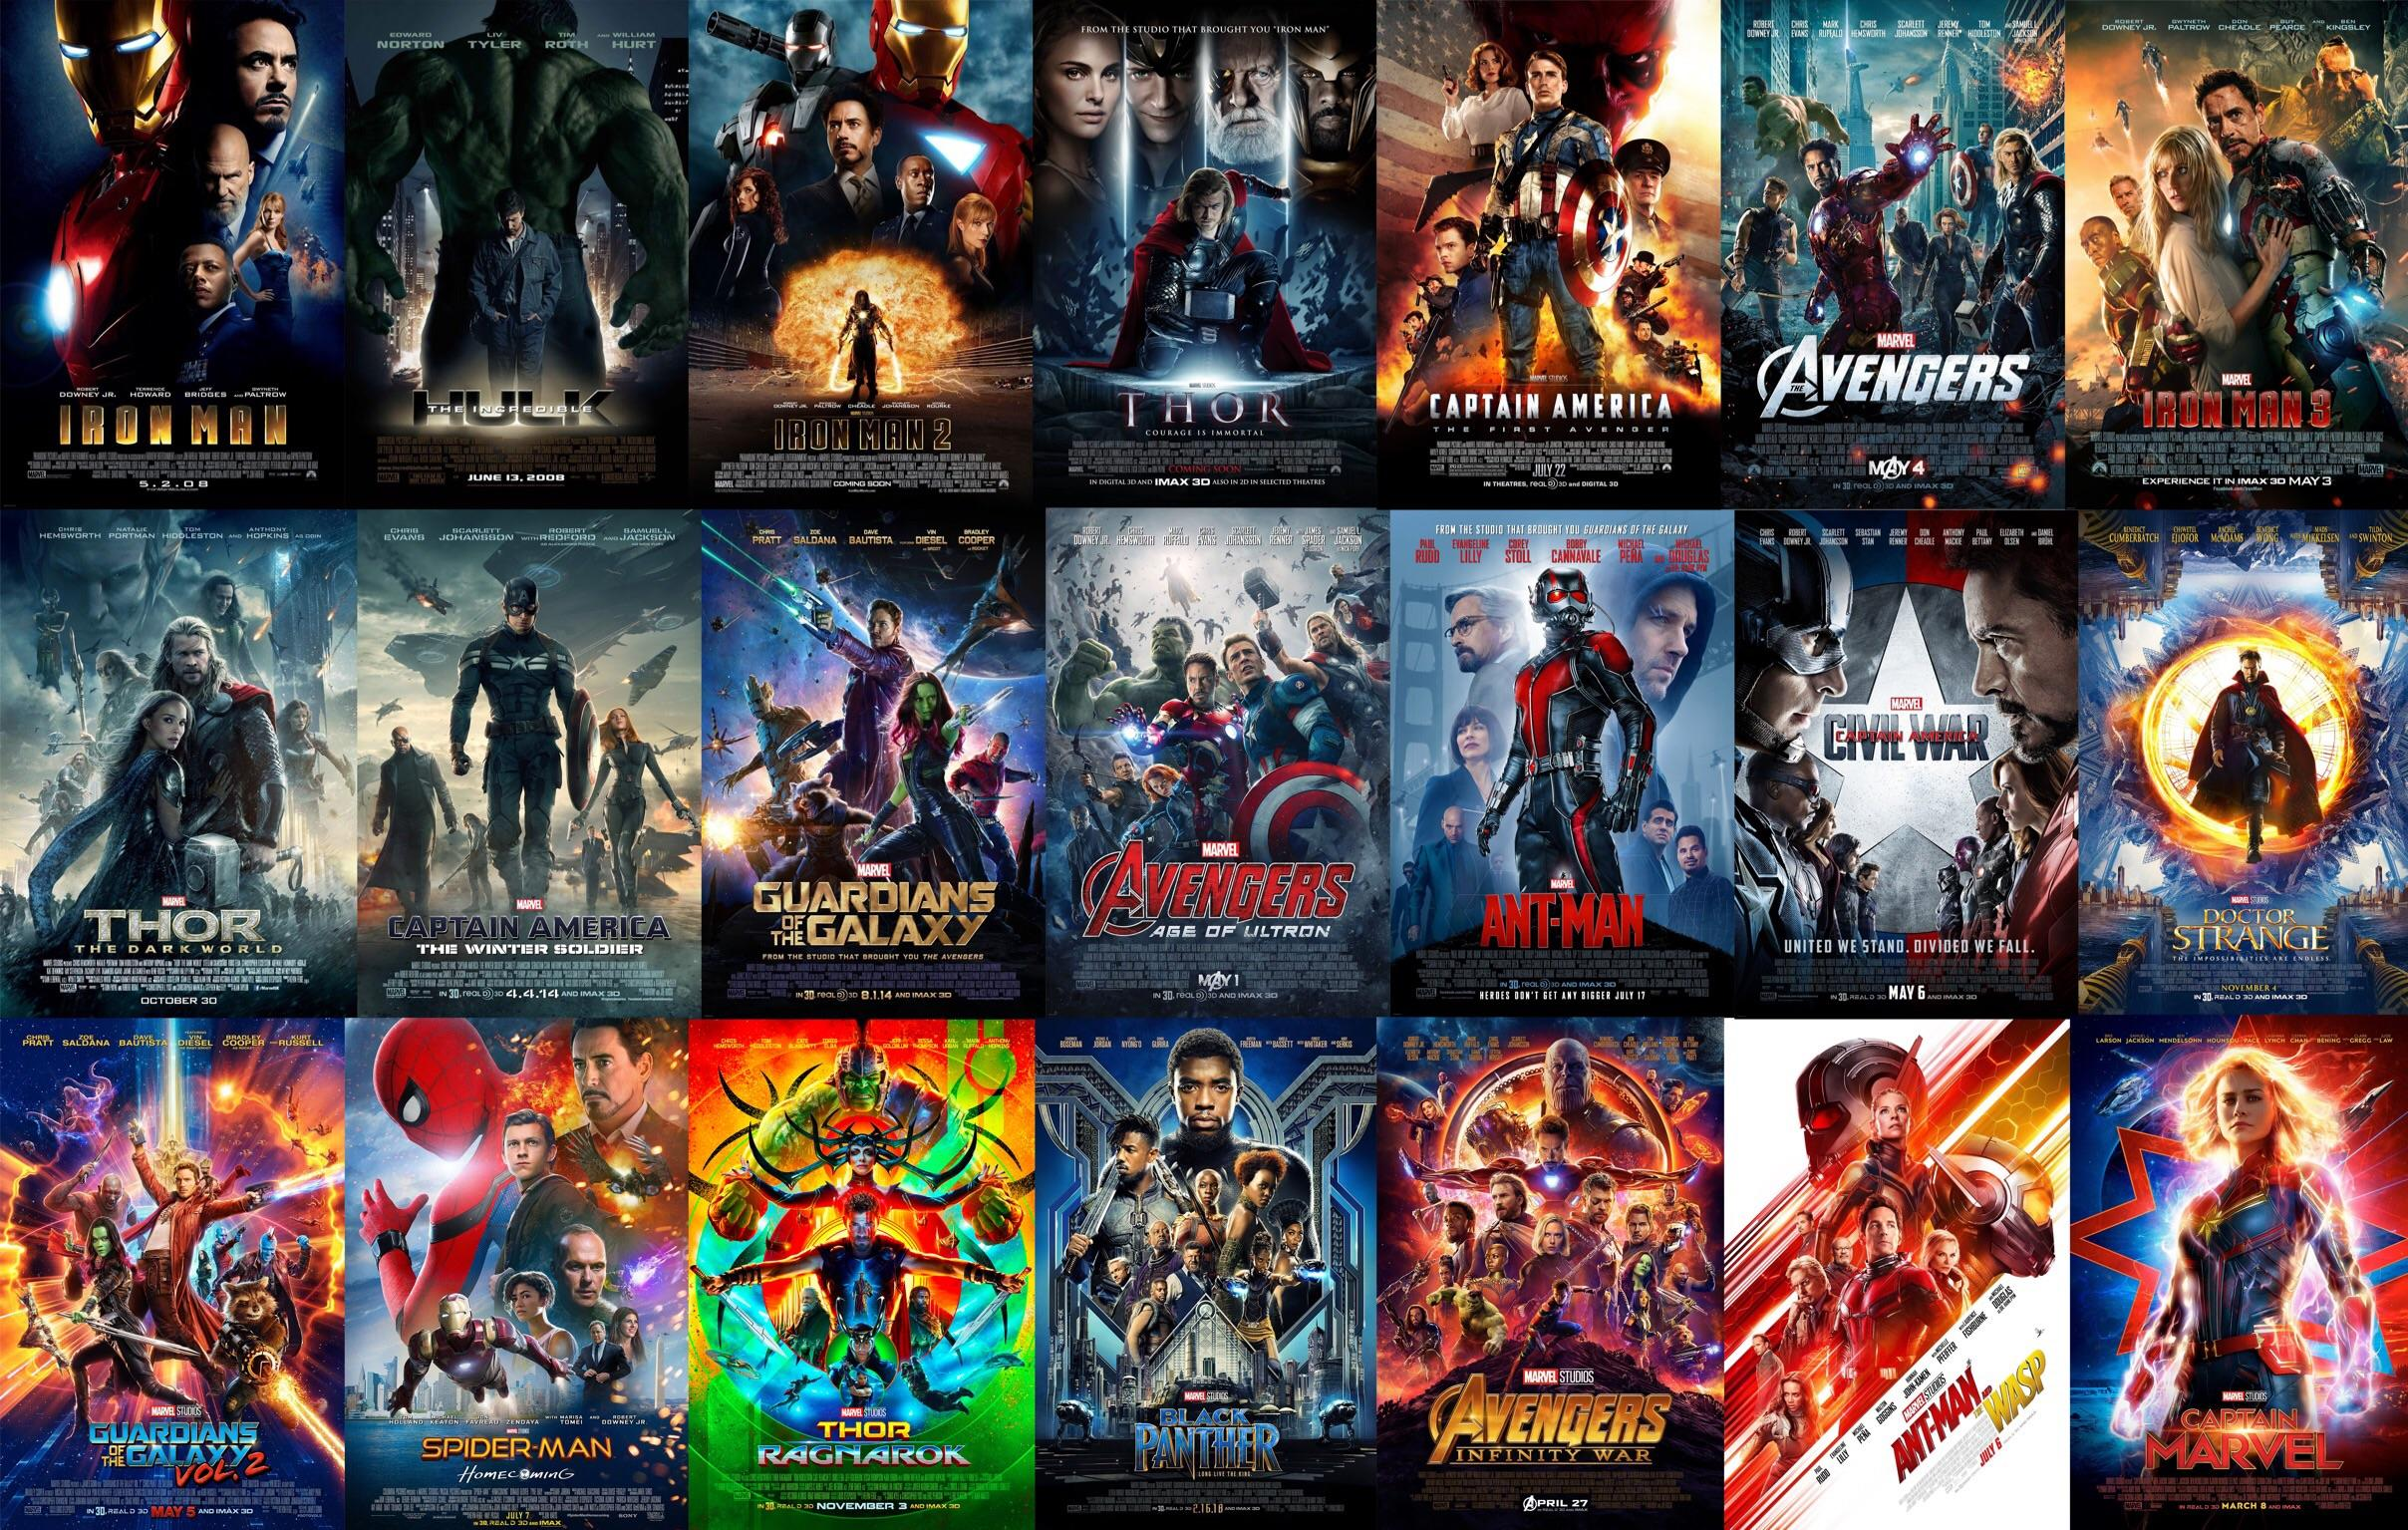
\includegraphics[width=\textwidth]{static/MCU.jpg}
    \end{minipage}
\end{frame}

\begin{frame}
    \begin{minipage}{.49\textwidth}
        \centering
        \textbf{\Large{23 movies}}
    \end{minipage} \pause
    \begin{minipage}{.49\textwidth}
        \centering
        \textbf{\Large{8000+ characters}}
    \end{minipage}
\end{frame}

\begin{frame}
    \centering
    \textbf{\large{Who is the most important character in the MCU?}}
\end{frame}

\begin{frame}
    \centering
    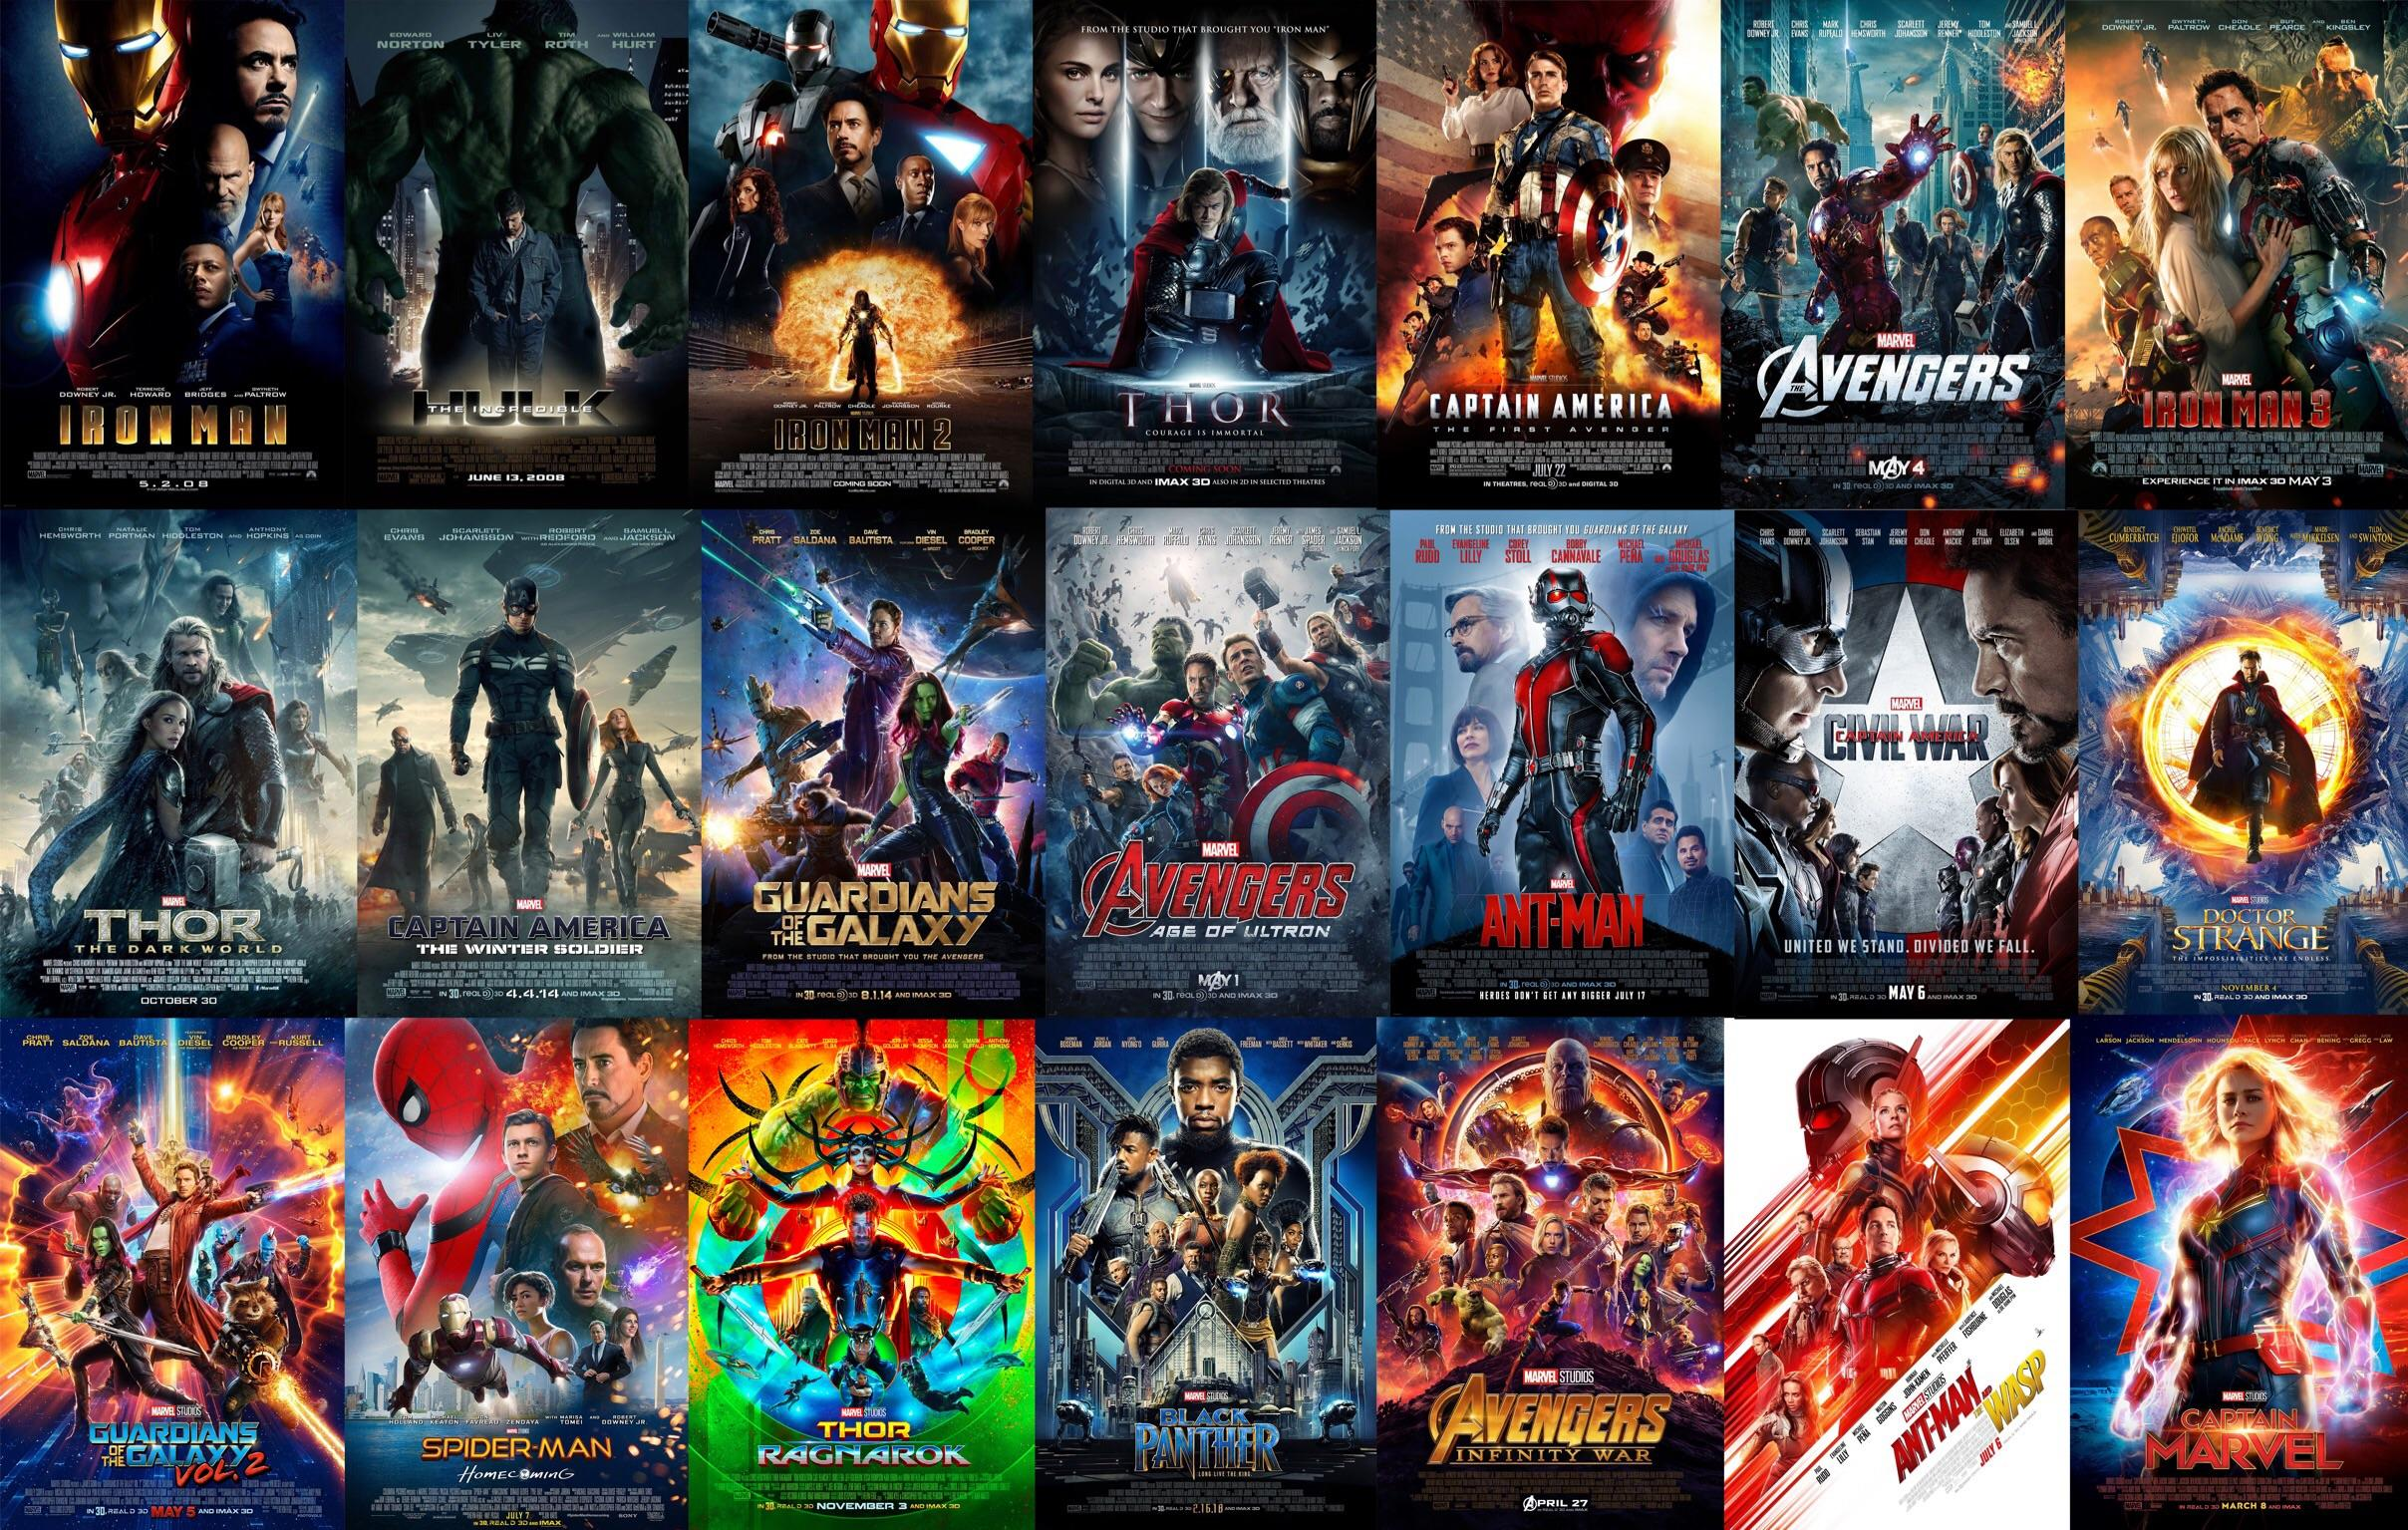
\includegraphics[width=\textwidth]{static/MCU.jpg}
\end{frame}

\begin{frame}
    \centering
    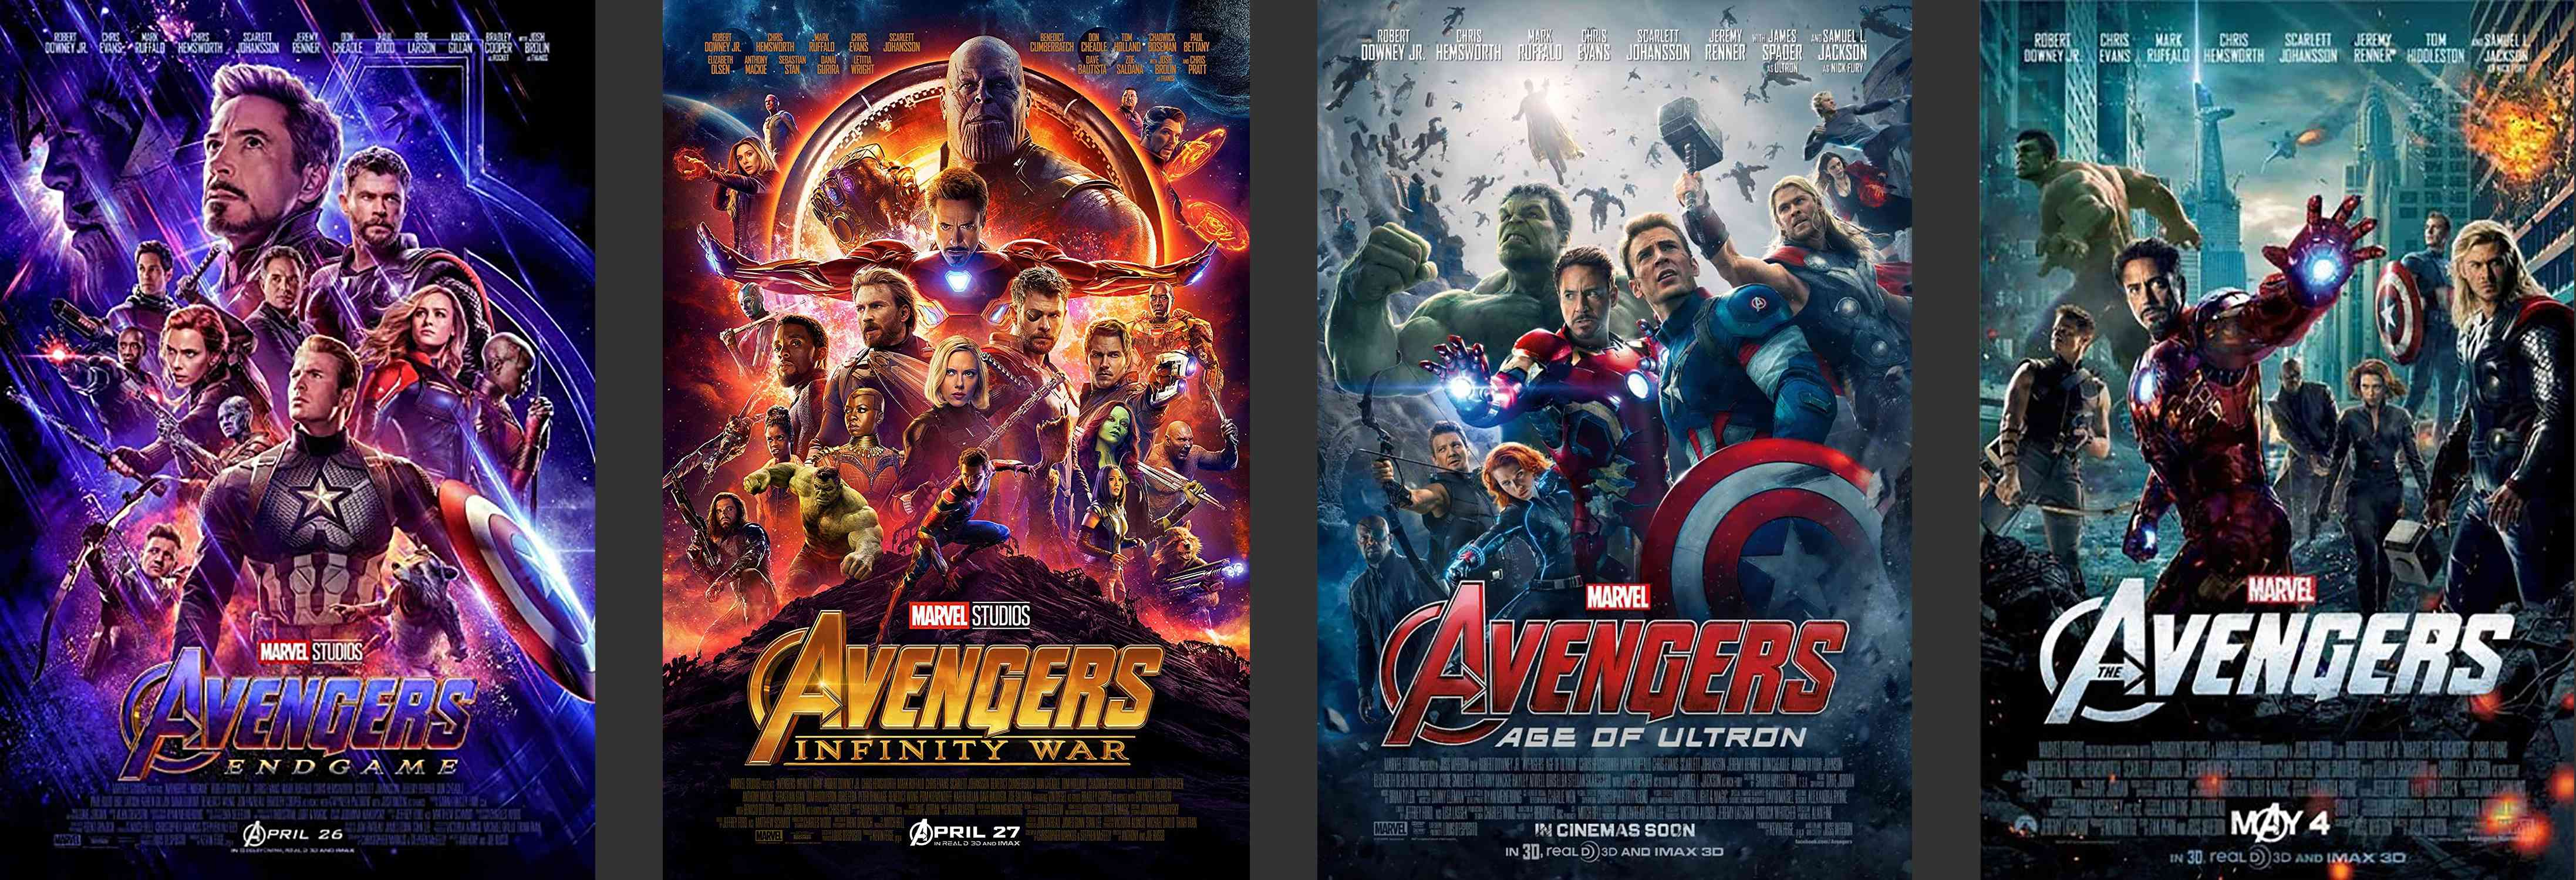
\includegraphics[width=\textwidth]{static/avenger.jpg}
\end{frame}

\begin{frame}
    \centering
    \textbf{\large{Which character has the most lines?}}
\end{frame}

\begin{frame}
    \centering
    \includestandalone[width=\textwidth]{static/sentence}
\end{frame}


\begin{frame}
    \centering
    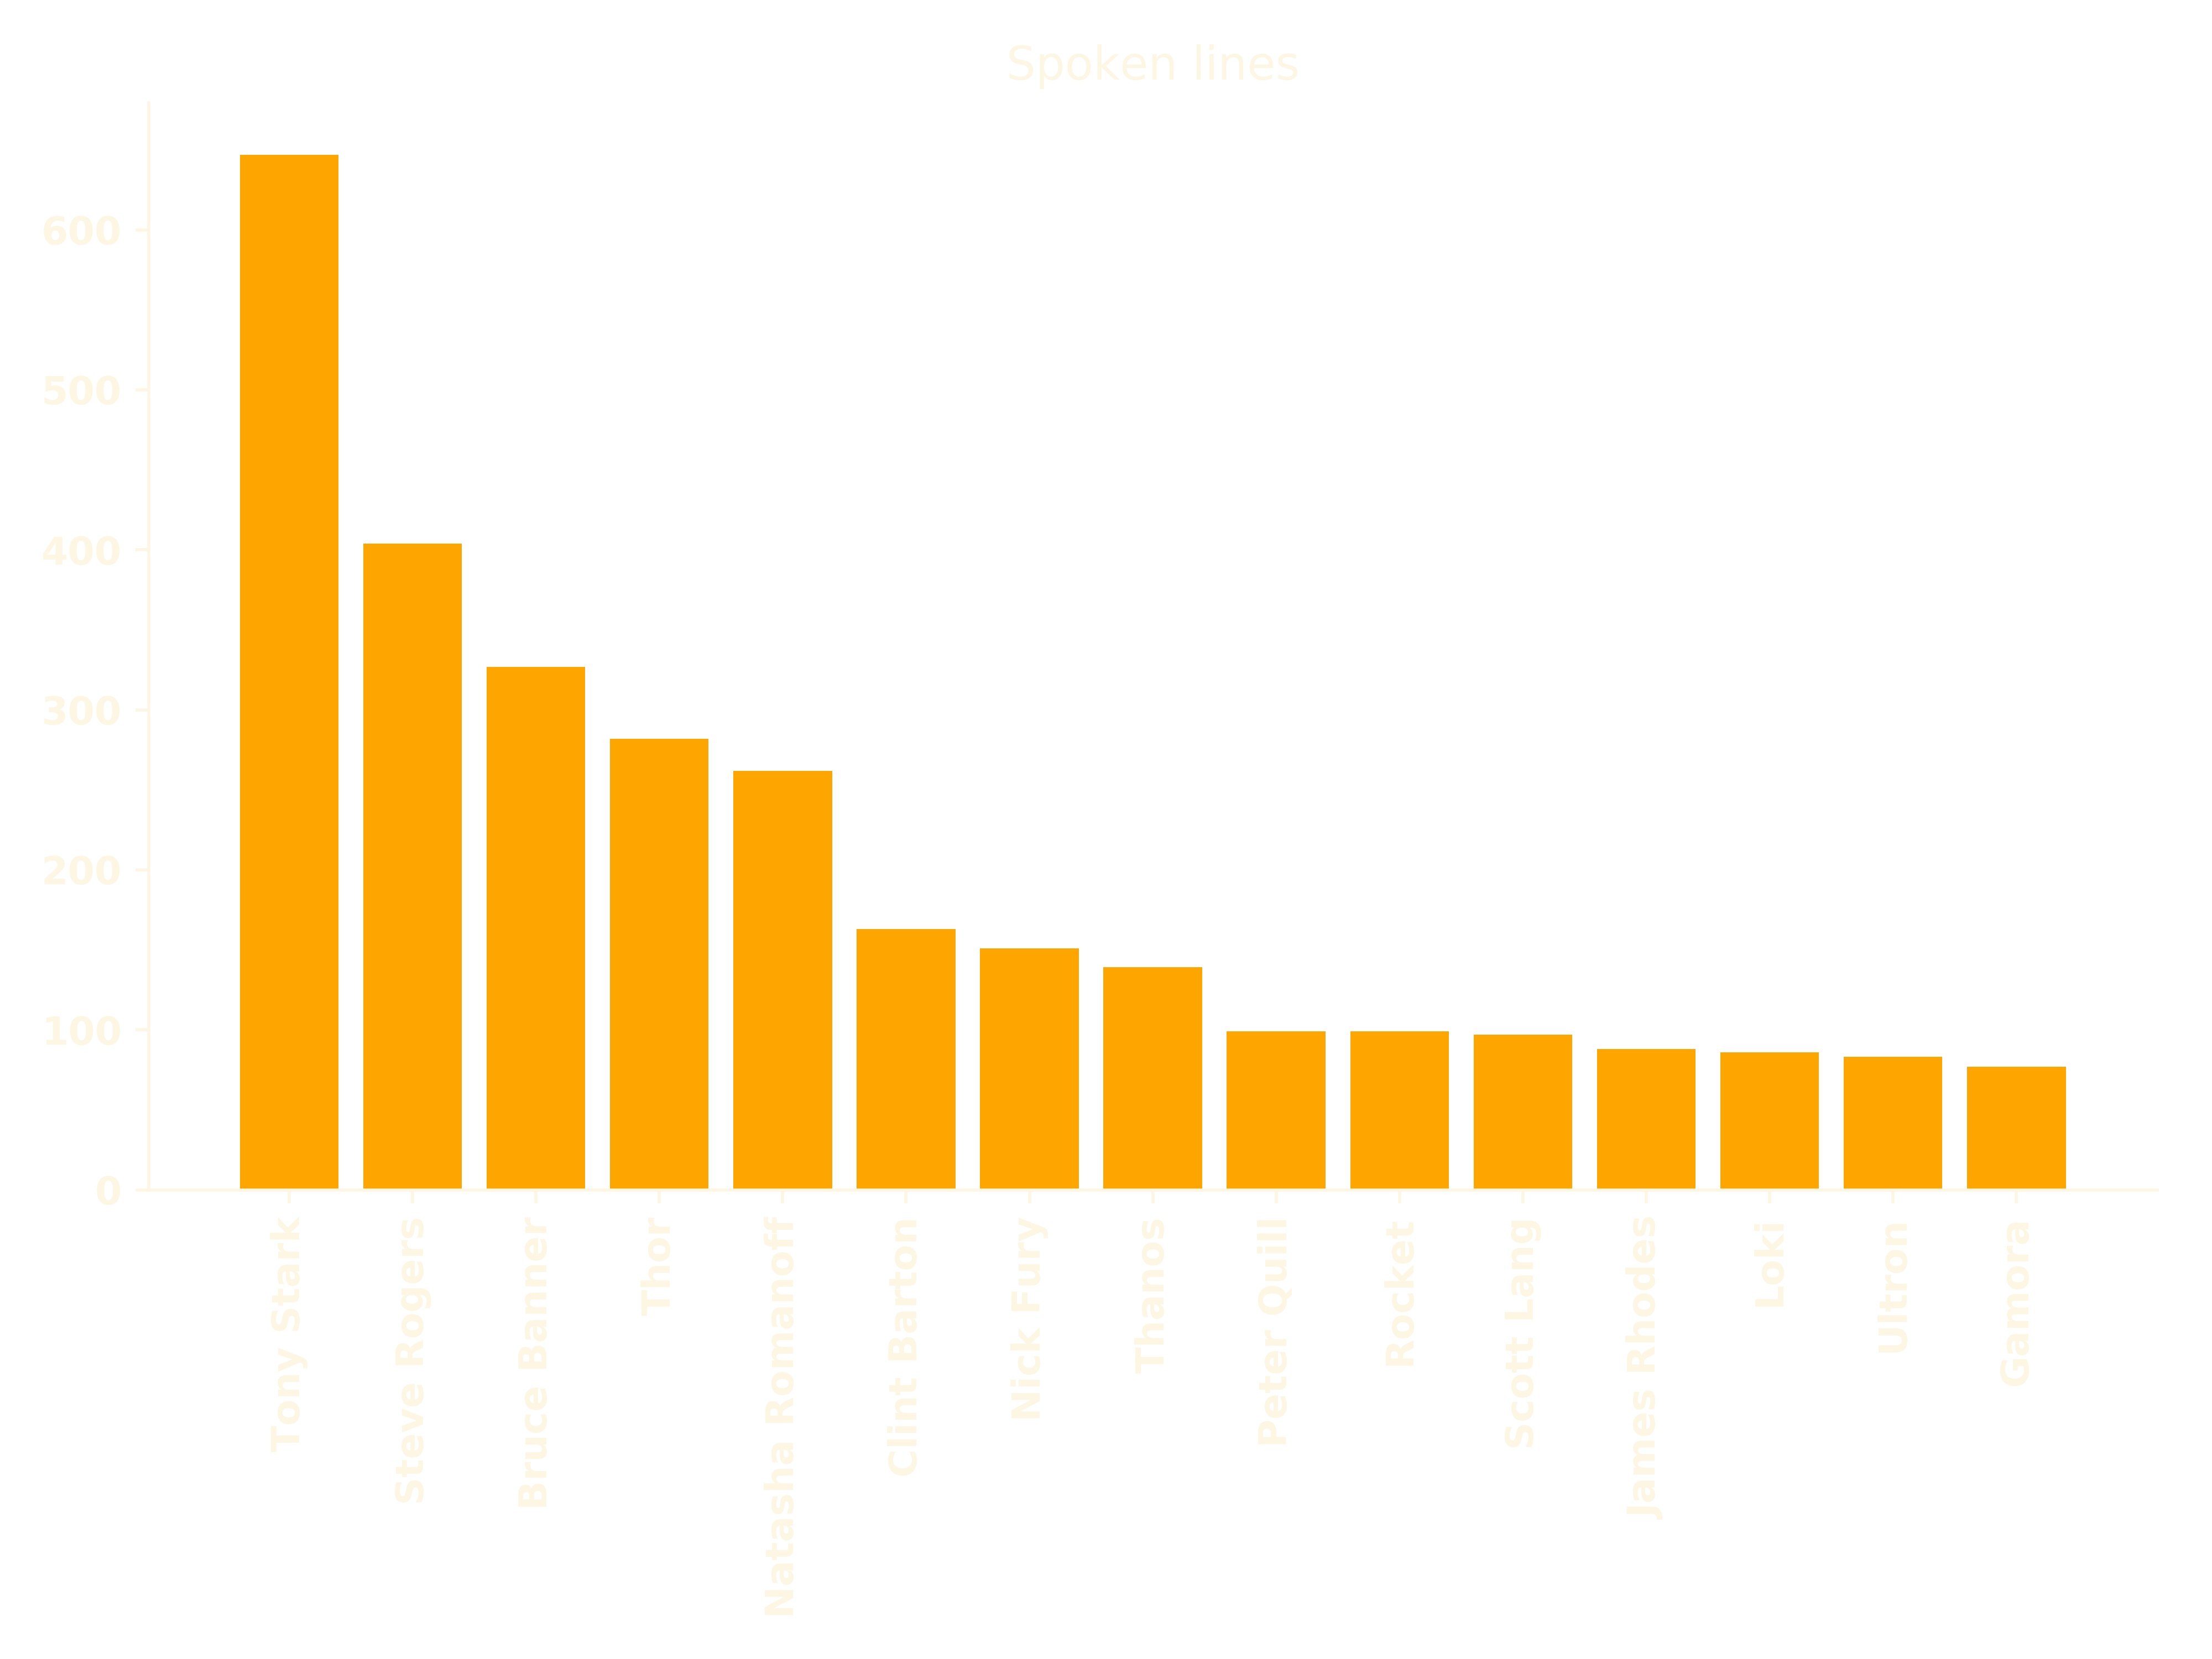
\includegraphics[width=\textwidth]{static/spoken.png}
\end{frame}


\begin{frame}
    \centering
    \includestandalone[width=\textwidth]{static/mention}
\end{frame}

\begin{frame}[fragile]
	\begin{minted}
    [
    framesep=4mm,
    baselinestretch=1.2,
    bgcolor=DarkGray,
    fontsize=\scriptsize
    ]
    {python}
import spacy
nlp = spacy.load("en_core_web_sm")

def identify_names(text):

... doc = nlp(text)
... names = [ent.text for ent in doc.ents if ent.label_ == 'PERSON']

... return names
\end{minted}
\end{frame}

\begin{frame}
    \centering
    \textbf{\large{Which character is mentioned the most?}}
\end{frame}

\begin{frame}
    \centering
    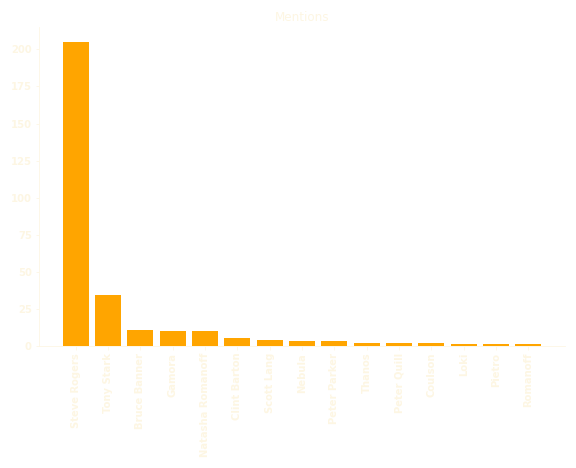
\includegraphics[width=\textwidth]{static/mentions.png}
\end{frame}

\begin{frame}
    \centering
    \includestandalone[width=\textwidth]{static/stones}
\end{frame}

\begin{frame}
    \centering
    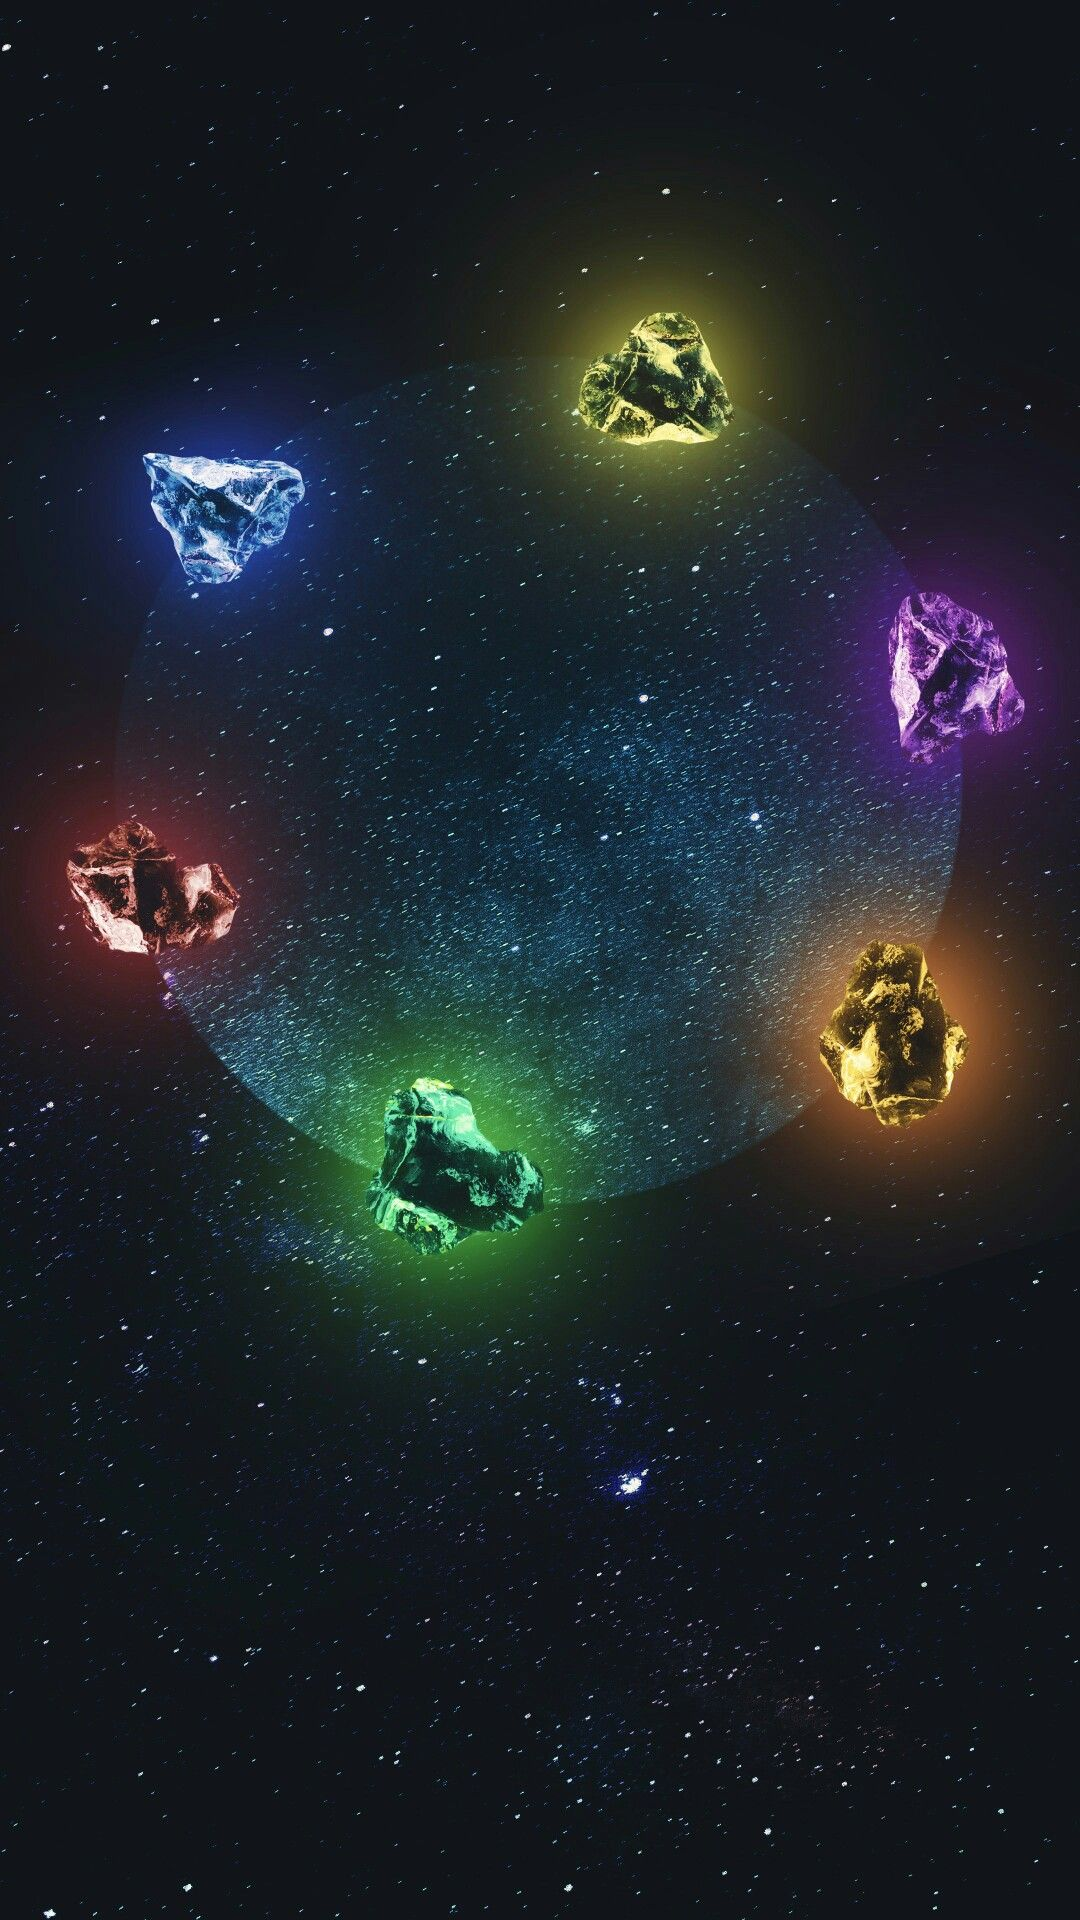
\includegraphics[width=.4\textwidth]{static/infinity_stones.jpg}
\end{frame}

\begin{frame}[fragile]
	\begin{minted}
    [
    framesep=4mm,
    baselinestretch=1.2,
    bgcolor=DarkGray,
    fontsize=\scriptsize
    ]
    {python}
import spacy
nlp = spacy.load("en_core_web_sm")

def identify_names_and_stones(text):

... doc = nlp(text)
... names = [ent.text for ent in doc.ents if ent.label_ == 'PERSON']
... stones = [word.text for word in doc 
...           if word.text in names_lookup['Infinity stones']]

... return names + stones
\end{minted}
\end{frame}

\begin{frame}
    \centering
    \textbf{\large{Which character interacts with the stones the most?}}
\end{frame}

\begin{frame}
    \centering
    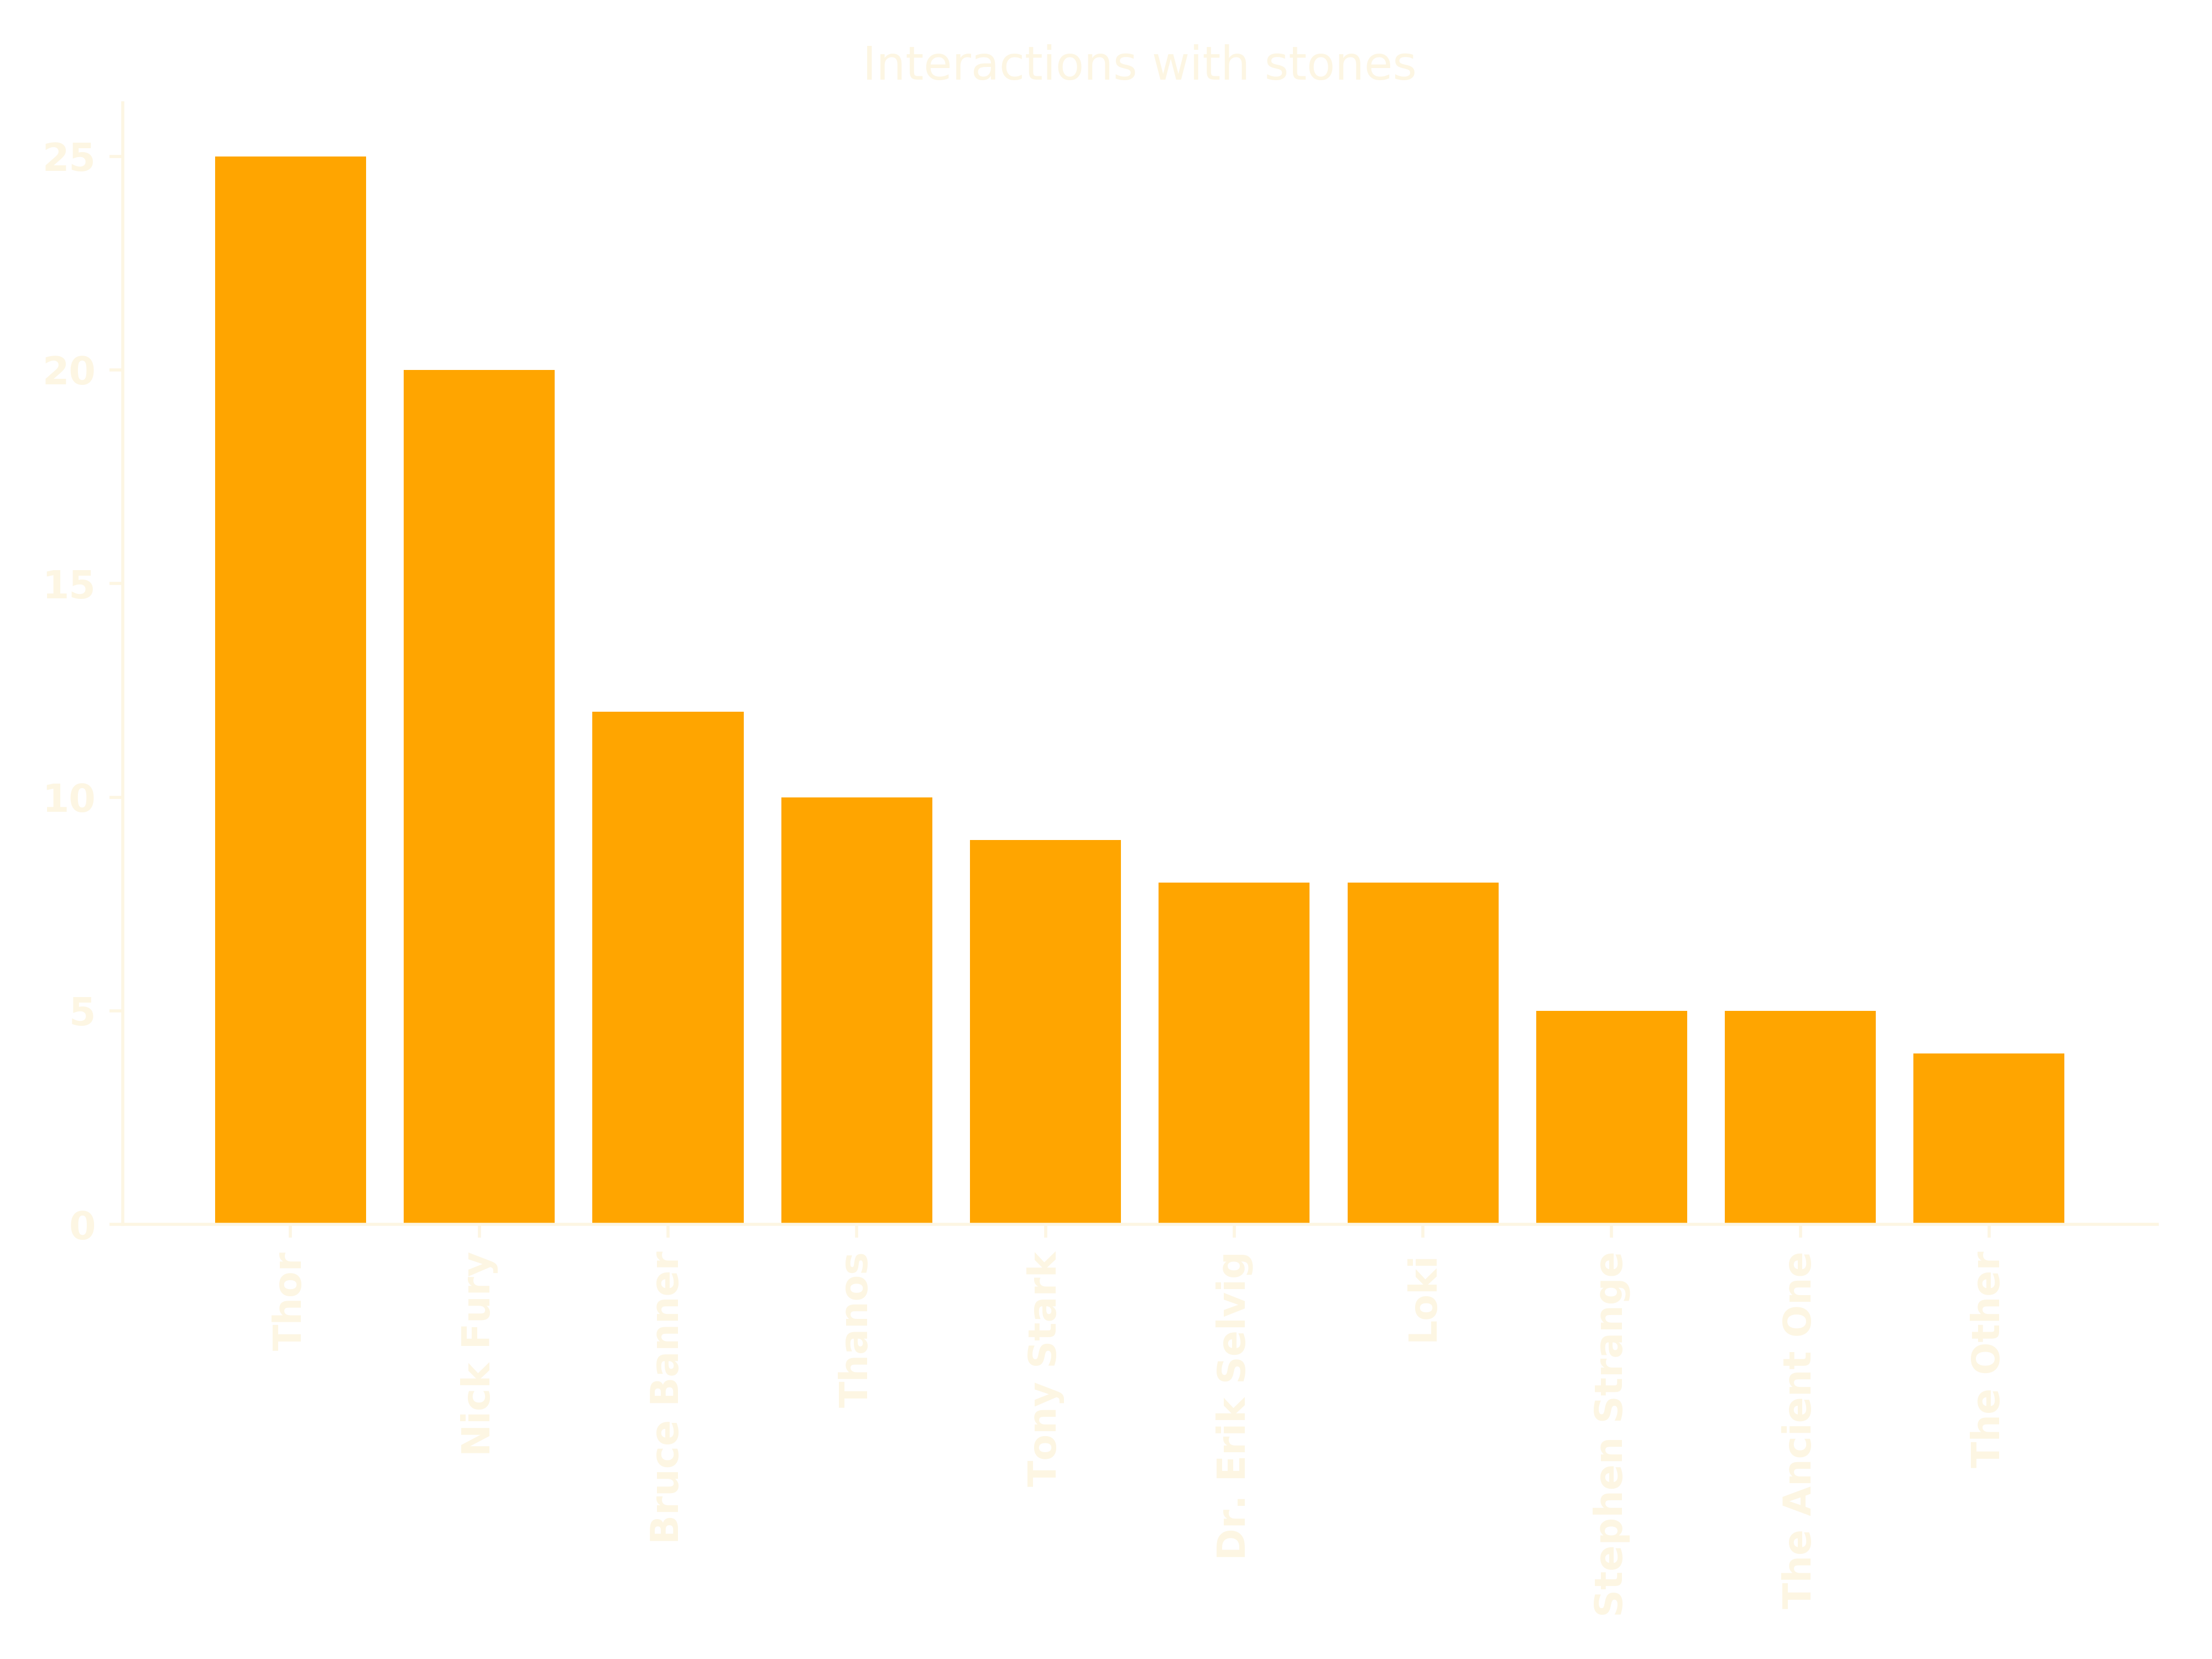
\includegraphics[width=\textwidth]{static/interactions_with_stones.png}
\end{frame}

\begin{frame}
    \hspace{.8cm} \LARGE{Social Network} \\

    \hspace{.8cm} \normalsize{1. A network of social interactions and}

    \hspace{1cm}\normalsize{personal relationships}
\end{frame}

\begin{frame}
    \centering
    \includestandalone[width=\textwidth]{static/connections}
\end{frame}

\begin{frame}
    \centering
    \includegraphics[width=.8\textwidth]{static/network.png}
\end{frame}

\begin{frame}
    \centering
    \textbf{\large{Who is the most connected character?}}
\end{frame}

\begin{frame}
    \centering
    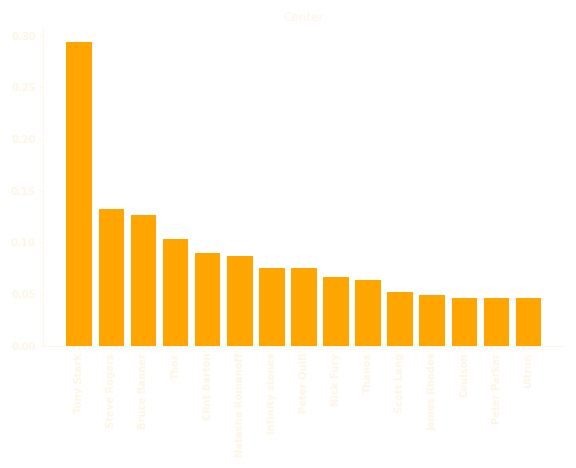
\includegraphics[width=\textwidth]{static/degree.png}
\end{frame}

\begin{frame}
    \centering
    \textbf{\large{Which character stands between others the most?}}
\end{frame}

\begin{frame}
    \centering
    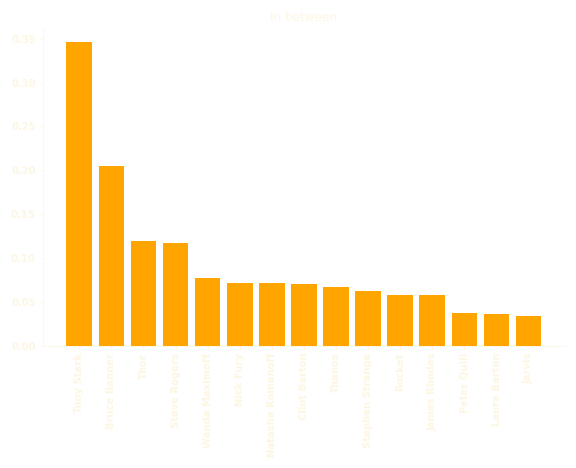
\includegraphics[width=\textwidth]{static/between.png}
\end{frame}

\begin{frame}
    \centering
    \textbf{\large{Which character is the most important based on Google?}}
\end{frame}

\begin{frame}
    \centering
    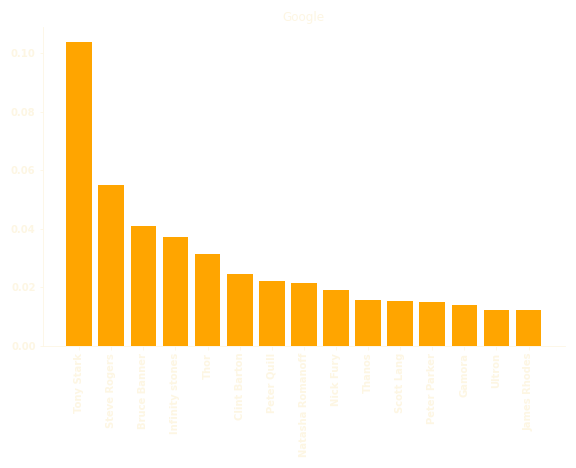
\includegraphics[width=\textwidth]{static/page_rank.png}
\end{frame}

\begin{frame}
    \centering
    \textbf{\large{Who is the most important character in the MCU?}}
\end{frame}

\begin{frame}
    \centering
    \textbf{\large{\st{Who is the most important character in the MCU?}}} \\ \vspace{10pt}
    \textbf{\large{What do we mean by the most important?}}
\end{frame}

\begin{frame}
    \centering
    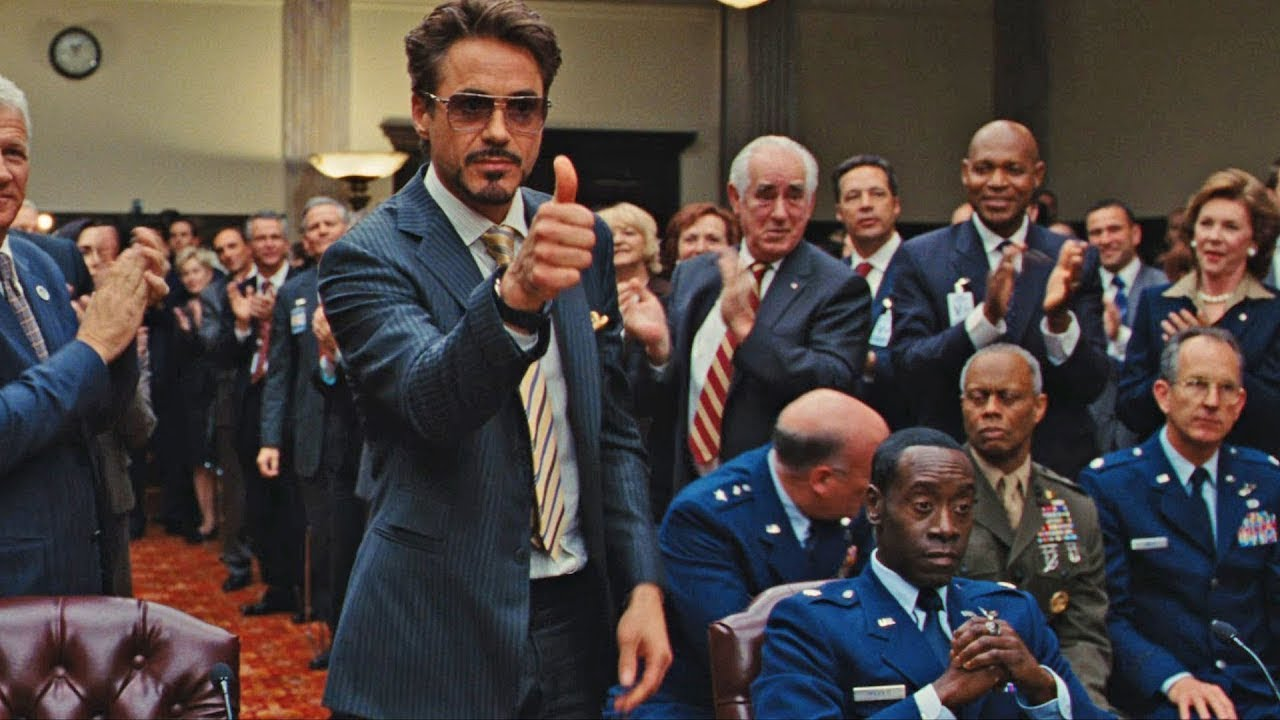
\includegraphics[width=\textwidth]{static/tony_stark.jpg}
\end{frame}

\begin{frame}
    \begin{center}
        \small
    \faTwitter \ @NikoletaGlyn \\
    \faGithub \ \url{https://github.com/Nikoleta-v3} \\
    \faGithub \ \url{https://github.com/Nikoleta-v3/avengers-analysis} \\ \vspace{1cm}



    \tiny{\url{https://medium.com/swlh/avengers-web-scraping-entity-extraction-and-network-graphs-in-python-ea6dc323eb7d}}
    \end{center}
\end{frame}

\end{document}